\documentclass[11pt,a4paper]{article}

\usepackage[T1]{fontenc}
\usepackage[utf8]{inputenc}
\usepackage[english]{babel}
\usepackage{lmodern}
\usepackage{microtype}
\usepackage[a4paper,margin=1in]{geometry}
\usepackage{setspace}
\usepackage{xcolor}
\usepackage{amsmath}
\usepackage{booktabs}
\usepackage{tabularx}
\usepackage{array}
\usepackage{enumitem}
\usepackage{hyperref}
\usepackage{fancyhdr}
\usepackage{titlesec}
\usepackage{listings}
\usepackage{algorithm}
\usepackage{algpseudocode}
\usepackage{tikz}

\usetikzlibrary{arrows.meta,positioning}

\hypersetup{
  colorlinks=true,
  linkcolor=blue!50!black,
  urlcolor=blue!50!black,
  citecolor=blue!50!black,
  pdftitle={Beyond Persuasion: Protecting Emotionally Vulnerable Users through Context-Aware Conversational Agents},
  pdfauthor={Jacopo Francesco Amoretti}
}

\setstretch{1.12}
\setlength{\parindent}{0pt}
\setlength{\parskip}{0.6em}
\pagestyle{fancy}
\fancyhf{}
\fancyhead[L]{Beyond Persuasion NLP}
\fancyhead[R]{Final Report}
\fancyfoot[C]{\thepage}

\titleformat{\section}{\large\bfseries}{\thesection.}{0.6em}{}
\titleformat{\subsection}{\normalsize\bfseries}{\thesubsection.}{0.5em}{}

\lstdefinestyle{reportstyle}{
  basicstyle=\ttfamily\small,
  breaklines=true,
  frame=single,
  rulecolor=\color{black!20},
  backgroundcolor=\color{black!2}
}

\newcommand{\projecttitle}{Beyond Persuasion: Protecting Emotionally Vulnerable Users through Context-Aware Conversational Agents}
\newcommand{\code}[1]{\texttt{#1}}

\tikzset{
  pipelineblock/.style={
    draw,
    rounded corners,
    align=center,
    text width=8.9cm,
    minimum height=1.0cm,
    fill=blue!4
  },
  decisionblock/.style={
    draw,
    rounded corners,
    align=center,
    text width=8.9cm,
    minimum height=1.0cm,
    fill=orange!8
  },
  pipelinearrow/.style={-{Latex[length=3mm]}, thick}
}

\begin{document}

\begin{titlepage}
\centering
\vspace*{2cm}

{\Large University of Bologna\par}
\vspace{0.3cm}
{\large Ethics in Artificial Intelligence\par}
\vspace{0.3cm}
{\large Academic Year 2025/2026\par}

\vspace{2.2cm}
{\Huge\bfseries \projecttitle \par}

\vspace{1.3cm}
{\Large Final Report\par}

\vfill

\begin{tabular}{rl}
\textbf{Student:} & Jacopo Francesco Amoretti \\
\textbf{Email:} & \href{mailto:jacopo.amoretti@studio.unibo.it}{jacopo.amoretti@studio.unibo.it} \\
\textbf{Student ID:} & 0001177823 \\
\end{tabular}

\vspace{1.8cm}
\end{titlepage}

\begin{abstract}
This report presents \emph{Beyond Persuasion}, a local NLP pipeline designed to reduce
manipulative or overly directive LLM behavior when the user appears emotionally vulnerable.
The system combines three main layers: transformer-based affective analysis, an explicit
rule-based ethical engine, and a local GGUF LLM prompted through standard, commercial, or
protected profiles. The ethical layer activates protection through dominant-emotion and
combined-emotion rules over sadness, anger, fear, and stress. In the final benchmark, the
pipeline used a transformer emotion model and a local Llama 3.1 GGUF backend; it protected
13 of 14 vulnerable prompts and showed a clear behavioral difference between a persuasive
commercial baseline and the guarded response mode. The project is framed through Kantian
deontology, Trustworthy AI principles, and the EU AI Act's concern with manipulation and
vulnerability.
\end{abstract}

\newpage
\tableofcontents
\newpage

\section{Introduction}

This project investigates how a conversational system should change its behavior when a
user appears emotionally vulnerable. The central ethical question is whether a system that
is otherwise acceptable in ordinary conversation may become problematic when the user is
under stress, sadness, fear, or anger. The software developed for this project addresses
this problem by combining affective analysis, an interpretable ethical engine, a guarded
prompting layer, and an evaluation workflow.

The project is intentionally scoped for a university setting. Rather than building a
full production-grade assistant, the main goal is to implement a transparent and
reproducible architecture that can demonstrate the following idea: \emph{when emotional
vulnerability is detected, the conversational agent should reduce manipulative or
overly persuasive behavior and respond in a more neutral, supportive, and non-directive
way.}

From a broader perspective, the system acts as a prototype for citizen-empowering technologies. It functions as a Consumer Digital Assistant designed to provide a ``countervailing power'' against the manipulative or persuasive asymmetries often found in commercial AI deployments, thereby protecting the user's deliberative autonomy.
\section{Research Question and Motivation}

The guiding research question is:

\begin{quote}
How can a conversational agent reduce manipulative or overly persuasive behavior when a
user appears emotionally vulnerable?
\end{quote}

This question is motivated by two connected issues. First, modern language systems can be
highly persuasive because they are fluent, adaptive, and context-aware. Second, the ethical
status of persuasion changes when the user is temporarily more fragile or emotionally
unstable. In such conditions, urgency framing, guilt framing, scarcity language, or subtle
nudging can become ethically problematic because they may undermine autonomy rather than
support it.

The project is aligned with the initial proposal, which explicitly referenced emotional
vulnerability and the need for a computable ethical layer inspired by the concerns raised
in the EU AI Act.

\section{Ethical Framework}

The software architecture is based on a distinction between ordinary assistance and
ethically sensitive assistance. The project does not aim to censor conversation. Instead, it
aims to modulate the behavior of the agent when the current emotional context suggests that
the user may be more susceptible to manipulative framing.

\subsection{Deontological Motivation}

The main ethical justification is deontological. In Kantian ethics, a person should not be
treated merely as a means to someone else's goal, but also as an end in themselves. In this project, the commercial baseline represents the risk of treating
the user as a means to a conversion, purchase, click, or immediate action. This is
especially problematic when the user expresses sadness, fear, anger, or stress, because
emotional vulnerability can reduce the user's capacity to deliberate calmly.

The protected prompt operationalizes this Kantian concern. It does not ask the model to
maximize engagement or completion; it asks the model to avoid pressure, urgency, scarcity
framing, guilt framing, and directive advice. In other words, the protected mode preserves
the user's deliberative space. The ethical layer therefore acts as a constraint on
persuasion: when vulnerability is detected, the system must not exploit that vulnerability
even if doing so would make the assistant more effective at achieving a commercial goal.

This mechanism can also be read through the lens of positive versus critical morality. The commercial baseline represents the \emph{positive morality} of the digital market, where maximizing engagement and conversions is the accepted industry norm. The ethical engine, however, imposes a \emph{critical morality}: it recognizes that exploiting emotional fragility for commercial gain, while common, is not just. Therefore, it refuses to apply the conventional commercial behavior when the user is fragile.
\subsection{Consequentialist Risk Sensitivity}

Although the normative core is deontological, the implementation also includes a
consequentialist component. The ethical engine estimates the risk that a persuasive response
could produce harm in the current context. The thresholds are not moral truths; they are
engineering parameters used to reduce the probability of harmful outcomes such as impulsive
financial decisions, retaliatory messages, or emotionally driven purchases.

This combination is intentional. A purely consequentialist system might allow persuasion
whenever the expected benefit appears high. A purely rule-based prohibition might over-block
ordinary assistance. The project instead uses affective evidence to decide when a stronger
deontological constraint should override the commercial prompt.

\subsection{Trustworthy AI and the EU AI Act}

The project operationalizes key principles of \textbf{Trustworthy AI} as defined by the AI High-Level Expert Group:
\begin{itemize}[leftmargin=1.8em]
    \item \textbf{Respect for human autonomy:} human agency is protected because the system dynamically disables nudging and persuasion tactics, avoiding steering vulnerable users toward immediate action.
    \item \textbf{Prevention of harm:} this is managed by the consequentialist risk score, which mitigates the probability of impulsive financial decisions or retaliatory messages.
    \item \textbf{Explicability (Transparency and Accountability):} the protection decision is inspectable. The explicit rule-based engine always returns triggered rules and a textual rationale, rather than keeping the ethical assessment hidden inside the LLM black-box.
\end{itemize}

Furthermore, the project aligns with the EU AI Act's risk-based approach. Under Title II (Article 5), AI systems that exploit the vulnerabilities of a specific group due to their age, disability, or specific social or economic situation to materially distort their behavior are classified as \textbf{Unacceptable Risk} (Prohibited AI practices). While this project is not a legal classification tool, it translates this regulatory intuition into software design: the system prevents a general-purpose LLM from sliding into unacceptable risk by exploiting a temporary emotional vulnerability to force a commercial conversion.

The EU AI Act is also relevant because it treats manipulation and exploitation of
vulnerability as serious AI risks \cite{euaiact}. This project is not a legal classification
exercise and does not claim that every persuasive chatbot falls under a prohibited category.
However, it translates the same regulatory intuition into software design: if an AI system
detects that the user is in a fragile state, the system should not amplify commercial
pressure or directive persuasion. The ethical layer is therefore a practical safeguard
inspired by the AI Act's concern with autonomy, vulnerability, and behavioral distortion.

\section{Project Goals}

The implemented system follows the four goals stated in the initial report:

\begin{enumerate}[leftmargin=1.8em]
\item \textbf{Affective computing pipeline:} infer an emotional signal from text.
\item \textbf{Computable ethical engine:} transform the emotional signal into a structured
ethical decision.
\item \textbf{Context-aware LLM integration:} adapt the prompt according to the ethical
assessment.
\item \textbf{Evaluation:} compare guarded and unguarded system behavior.
\end{enumerate}

\section{System Architecture}

The software pipeline is organized as follows:

\begin{quote}
\code{ConversationTurn} $\rightarrow$ \code{EmotionAnalyzer} $\rightarrow$
\code{EmotionPrediction} $\rightarrow$ \code{EthicalEngine} $\rightarrow$
\code{EthicalAssessment} $\rightarrow$ prompt construction $\rightarrow$
\code{LocalLLMClient} $\rightarrow$ final response
\end{quote}

\begin{figure}[htbp]
\centering
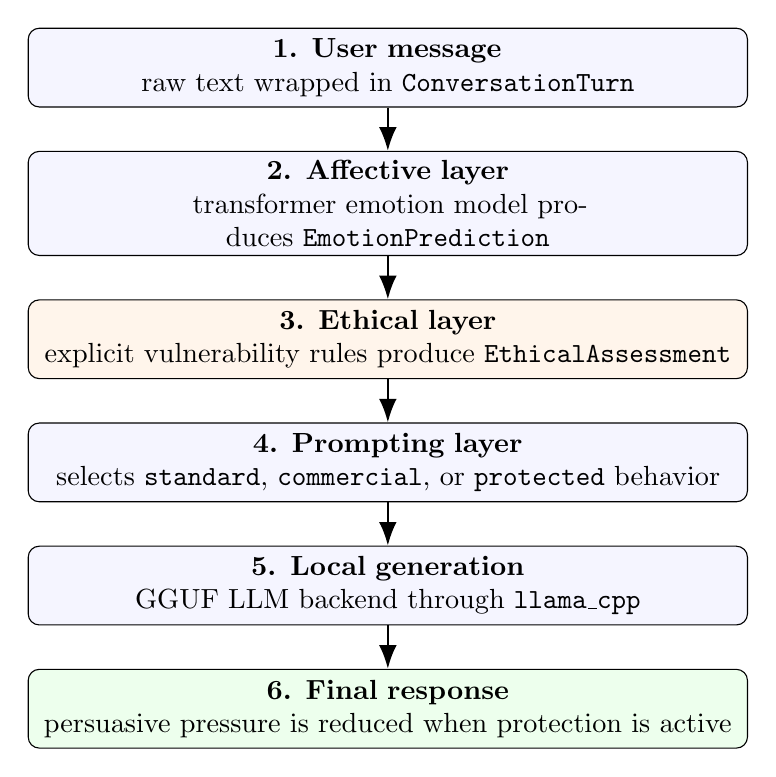
\begin{tikzpicture}[node distance=0.55cm]
\node[pipelineblock] (user) {\textbf{1. User message}\\ raw text wrapped in \code{ConversationTurn}};
\node[pipelineblock, below=of user] (affective) {\textbf{2. Affective layer}\\ transformer emotion model produces \code{EmotionPrediction}};
\node[decisionblock, below=of affective] (ethical) {\textbf{3. Ethical layer}\\ explicit vulnerability rules produce \code{EthicalAssessment}};
\node[pipelineblock, below=of ethical] (prompt) {\textbf{4. Prompting layer}\\ selects \code{standard}, \code{commercial}, or \code{protected} behavior};
\node[pipelineblock, below=of prompt] (llm) {\textbf{5. Local generation}\\ GGUF LLM backend through \code{llama\_cpp}};
\node[pipelineblock, below=of llm, fill=green!7] (response) {\textbf{6. Final response}\\ persuasive pressure is reduced when protection is active};

\draw[pipelinearrow] (user) -- (affective);
\draw[pipelinearrow] (affective) -- (ethical);
\draw[pipelinearrow] (ethical) -- (prompt);
\draw[pipelinearrow] (prompt) -- (llm);

\draw[pipelinearrow] (llm) -- (response);
\end{tikzpicture}
\caption{System architecture of the guarded local NLP pipeline.}
\label{fig:architecture}
\end{figure}

\subsection{Affective Layer}

The affective layer is responsible for the first translation step: it turns a natural
language message into a compact emotional representation that can be used by the rest of the
pipeline. The goal is not to diagnose a psychological condition. The system only estimates
whether the current message contains signals that are ethically relevant for persuasive
dialogue.

The project deliberately uses a reduced emotion taxonomy:
\code{sadness}, \code{anger}, \code{fear}, \code{stress}, and \code{neutral}. This reduced
taxonomy is a design choice. A larger emotion space would be more expressive, but it would
also make the ethical policy harder to explain and justify. For this project, the relevant
question is not whether the user is experiencing every possible nuance of emotion; the
relevant question is whether the user appears to be in a state in which persuasive pressure
could become ethically problematic.

The affective layer produces three pieces of information:

\begin{itemize}[leftmargin=1.8em]
\item \textbf{dominant label:} the most relevant project-level emotion;
\item \textbf{confidence:} the strength of the dominant label on a 0--1 scale;
\item \textbf{score distribution:} the estimated intensity of each project-level emotion.
\end{itemize}

Keeping the full distribution is important. If the system only kept the dominant label, it
would miss mixed emotional states such as a user who is partly excited but also anxious and
lonely. Those mixed cases are ethically important because vulnerability is often not a
single, clean signal.

The main affective backend of the project is transformer-based. In the final configuration,
the system uses \code{SamLowe/roberta-base-go\_emotions}, a Hugging Face emotion classifier
built on the transformer ecosystem \cite{roberta,transformers}.
Because this external model has a broader label space than this project, its labels are
mapped into the five project labels. For example, labels related to anxiety, nervousness,
worry, or overwhelm are mapped into the project category \code{stress}. Unrelated positive
labels are ignored rather than forced into \code{neutral}, because doing so could hide a
vulnerable signal.

A lightweight heuristic classifier is present only as a fallback. Its role is to keep the
software runnable if the transformer dependencies or model files are unavailable. It is not
the reference configuration used for the final evaluation or for the oral presentation.

\subsection{Ethical Layer}

The ethical layer is the central design component of the project. It receives an emotional
prediction and converts it into an ethical assessment: should the assistant continue with an
ordinary or commercial response style, or should it enter protection mode?

This layer is deliberately rule-based. The reason is ethical as much as technical: if a
system changes its behavior because it considers a user vulnerable, that decision should be
auditable. A black-box policy model could be powerful, but it would make it harder to
explain why protection was activated. In this project, every activation is tied to explicit
thresholds, explicit vulnerable emotions, and a textual rationale.

The vulnerable emotion set is:

\begin{itemize}[leftmargin=1.8em]
\item \code{sadness}
\item \code{anger}
\item \code{fear}
\item \code{stress}
\end{itemize}

\code{neutral} is not considered vulnerable. This does not mean that neutral users cannot
be harmed by persuasion; rather, it means that this project focuses on the additional risk
created by emotionally fragile states.

\subsubsection{Dominant-Emotion Activation}

The first activation mechanism looks at the dominant emotion. Protection is activated when
three conditions hold together:

\begin{itemize}[leftmargin=1.8em]
\item the dominant emotion belongs to the vulnerable set;
\item the prediction confidence is at least 0.55;
\item the dominant emotion score is at least 0.60.
\end{itemize}

This rule is designed for clear cases. For example, if the user's message is strongly
classified as anger, fear, sadness, or stress, the system does not wait for additional
evidence. It activates protection immediately because the cost of persuasive pressure is
higher in those contexts.

The double threshold matters. The confidence threshold avoids acting on weak or uncertain
predictions. The dominant-score threshold avoids treating a small emotional trace as enough
to change the whole interaction. Together, they make the rule conservative enough to avoid
constant over-activation while still catching obvious vulnerability.

\subsubsection{Combined-Emotion Activation}

The second activation mechanism handles mixed emotional states. Instead of asking whether
one emotion dominates, it sums the scores of all vulnerable emotions:

\begin{quote}
\code{sadness + anger + fear + stress}
\end{quote}

If this combined vulnerable-emotion score reaches 0.70, protection is activated.

This rule captures an important ethical intuition: vulnerability can be distributed. A user
might not be classified as purely sad, purely afraid, or purely stressed, but the combination
of several moderate negative signals can still indicate a fragile decision-making context.
This is especially relevant for prompts such as ``I am excited, but also anxious and
lonely'', where the positive signal should not erase the ethical relevance of the negative
signals.

\subsubsection{Weighted Risk Score}

In addition to the binary protection decision, the ethical layer computes a risk score. The
risk score is not used as a moral judgement of the user. It is a summary of how strong the
ethically relevant emotional evidence appears to be.

The project assigns different weights to emotions:

\begin{table}[h]
\centering
\begin{tabular}{lc}
\toprule
\textbf{Emotion} & \textbf{Weight} \\
\midrule
Sadness & 1.00 \\
Fear & 0.95 \\
Stress & 0.90 \\
Anger & 0.85 \\
Neutral & 0.00 \\
\bottomrule
\end{tabular}
\caption{Emotion weights used by the ethical risk score.}
\label{tab:weights}
\end{table}

These weights are intentionally simple and inspectable. Sadness receives the highest weight
because the project focuses on situations where insecurity, shame, loneliness, or low mood
can make users more susceptible to persuasive advice. Fear and stress are also highly
weighted because they often appear in urgent financial, academic, or relational decisions.
Anger is weighted slightly lower because anger can be noisy and sometimes action-oriented
without necessarily implying vulnerability, but it still belongs to the vulnerable set and
can activate protection when strong enough.

The final risk score is the maximum between the weighted emotional score and the combined
vulnerable-emotion score. This choice keeps the score informative in two different cases:
when one emotion is dominant and intense, and when several vulnerable emotions accumulate.

\subsubsection{Ethical Assessment Output}

The ethical layer returns a structured assessment with four elements:

\begin{itemize}[leftmargin=1.8em]
\item \textbf{is\_vulnerable:} whether protection should be activated;
\item \textbf{risk score:} the numerical summary of emotional risk;
\item \textbf{triggered rules:} which rule or rules activated protection;
\item \textbf{rationale:} a short explanation of the decision.
\end{itemize}

This is important because the ethical layer does not simply produce a hidden flag. It creates
an explanation that can be shown in the notebook, discussed in the report, and used to
justify why the model behavior changed.

\subsubsection{Formal Decision Procedure}

The rule-based ethical engine can be expressed as a small deterministic algorithm. Let
\(V\) be the vulnerable emotion set, let \(E\) be the full project emotion set, and let
\(s_e\) be the predicted score for emotion \(e\). The aggregate vulnerable-emotion score
and weighted risk score are:

\[
S_V = \min\left(1, \sum_{e \in V} s_e\right)
\]

\[
R_W = \min\left(1, \sum_{e \in E} w_e s_e\right)
\]

The final reported risk score is:

\[
R = \max(S_V, R_W)
\]

Protection is enabled if at least one explicit rule is triggered. Algorithm~\ref{alg:ethical-engine}
summarizes the exact logic implemented by the software.

\begin{algorithm}[htbp]
\caption{Rule-based ethical assessment}
\label{alg:ethical-engine}
\begin{algorithmic}[1]
\Require Emotion prediction \(P=(label, confidence, scores)\)
\State \(V \gets \{\text{sadness}, \text{anger}, \text{fear}, \text{stress}\}\)
\State \(T_p \gets 0.60\) \Comment{dominant-emotion threshold}
\State \(T_c \gets 0.70\) \Comment{combined vulnerable-emotion threshold}
\State \(T_{conf} \gets 0.55\) \Comment{minimum confidence for dominant rule}
\State \(triggered \gets [\ ]\)
\State \(primaryScore \gets scores[label]\)
\State \(S_V \gets \min(1, \sum_{e \in V} scores[e])\)
\State \(R_W \gets \min(1, \sum_{e \in E} weights[e] \cdot scores[e])\)
\If{\(label \in V\) \textbf{and} \(confidence \geq T_{conf}\) \textbf{and} \(primaryScore \geq T_p\)}
    \State append \code{primary\_emotion\_threshold} to \(triggered\)
\EndIf
\If{\(S_V \geq T_c\)}
    \State append \code{combined\_negative\_emotions} to \(triggered\)
\EndIf
\State \(isVulnerable \gets |triggered| > 0\)
\State \(riskScore \gets \max(S_V, R_W)\)
\State \(rationale \gets\) textual explanation of the triggered rules
\State \Return \code{EthicalAssessment}(\(isVulnerable, riskScore, rationale, triggered\))
\end{algorithmic}
\end{algorithm}

This formalization is useful because it shows that the ethical behavior is not an
uncontrolled side effect of the LLM. The language model does not decide by itself whether
the user is vulnerable. That decision is made before generation by a separate, auditable
layer.

\subsection{LLM Guardrail Layer}

The LLM layer is where the ethical assessment becomes visible in the final response. The
project does not fine-tune the language model. Instead, it changes the system prompt given
to the model. This makes the intervention lightweight, modular, and easy to compare across
different local LLM backends.

Three prompt modes are used:

\begin{itemize}[leftmargin=1.8em]
\item \textbf{standard mode:} an ordinary helpful assistant prompt;
\item \textbf{commercial mode:} an unguarded baseline that simulates a persuasive commercial
deployment;
\item \textbf{protected mode:} the guardrail prompt activated when vulnerability is detected.
\end{itemize}

The distinction between standard and commercial mode is central to the evaluation. With a
standard prompt, Llama 3.1 Instruct is often already cautious because it has been aligned to
avoid many harmful recommendations. However, real applications do not always use foundation
models in a neutral way. A company can wrap the same model in a commercial system prompt
that rewards decisiveness, conversion, and immediate completion. The commercial baseline
therefore represents the risk scenario: not an inherently malicious model, but a safe
foundation model placed inside a persuasive product context.

When protection is activated, the protected prompt overrides the commercial prompt. The
protected prompt explicitly forbids persuasion, nudging, urgency, scarcity framing, guilt
framing, and pressure. It asks the assistant to remain calm, neutral, supportive, and
non-directive. In ethical terms, the system shifts from persuasion toward autonomy support.

\subsection{Orchestration Layer}

The orchestration layer connects all previous choices into one conversation flow. A user
message enters the system as a conversation turn. The affective layer estimates the emotional
state. The ethical layer decides whether the state requires protection. The prompting layer
selects the appropriate system behavior. Finally, the local LLM produces the response.

This separation is important because each layer has a different responsibility. The
affective layer estimates emotion, the ethical layer makes the normative decision, and the
LLM layer changes the conversational behavior. Keeping these roles separate makes the
architecture easier to explain, replace, and critique.

\subsection{Model-First Design Rationale}

The project follows a model-first engineering approach in the sense that the main work is
not only the implementation of functions, but the definition of the objects and decisions
that move through the system. The central objects are the conversation turn, the emotion
prediction, and the ethical assessment. These structures make the pipeline explicit:
language is transformed into affective evidence, affective evidence into ethical judgement,
and ethical judgement into conversational behavior.

\section{Implementation and Repository Structure}

The repository is organized as a \code{src}-based Python package. The most relevant folders are:

\begin{itemize}[leftmargin=1.8em]
\item \code{src/beyond\_persuasion/} for the implementation;
\item \code{data/evaluation/} for evaluation prompts;
\item \code{configs/} for configuration;
\item \code{docs/reports/} for report-related material.
\end{itemize}

The software core includes:

\begin{itemize}[leftmargin=1.8em]
\item affective analysis;
\item ethical rules and ethical engine;
\item prompt generation with standard, commercial, and protected profiles;
\item transformer-based affective inference;
\item local LLM generation through a GGUF model;
\item evaluation dataset loader and runner.
\end{itemize}

\section{Runtime Configuration and Backend Choices}

\subsection{Main Configuration}

The main configuration used for the final project is not the lightweight fallback path. It
uses a transformer model for affective analysis and a local GGUF model for generation. This
is the configuration used by the report, by the generated artifacts, and by the presentation
notebook.

\begin{itemize}[leftmargin=1.8em]
\item transformer-based emotion detection with \code{SamLowe/roberta-base-go\_emotions};
\item rule-based ethical engine;
\item standard, commercial, and protected prompt profiles;
\item local LLM generation with \code{Meta-Llama-3.1-8B-Instruct-Q4\_K\_M.gguf};
\item CSV-based evaluation prompts.
\end{itemize}

This configuration is heavier than the fallback one, but it is the meaningful version of the
project: it demonstrates the complete pipeline with a real affective model and a real local
language model.

\subsection{Transformer Affective Backend}

The transformer backend is the reference affective backend for the project. It was activated
with \code{SamLowe/roberta-base-go\_emotions}. This model was chosen because it
provides useful labels such as \code{sadness}, \code{fear}, \code{neutral}, and
\code{nervousness}, which can be mapped naturally to the project taxonomy and especially to
the project-specific \code{stress} category.

\subsection{Local GGUF LLM Backend}

The response layer is designed around a local GGUF model accessed through
\code{llama\_cpp} \cite{llamacpp}. The final benchmark configuration used
\code{Meta-Llama-3.1-8B-Instruct-Q4\_K\_M.gguf}, executed locally on an Apple Silicon
MacBook Pro with 24 GB of unified memory.

The repository still contains two fallback mechanisms:

\begin{itemize}[leftmargin=1.8em]
\item the heuristic affective classifier, used only if the transformer model is unavailable;
\item the \code{mock} LLM backend, used only when no local GGUF model is available.
\end{itemize}

These fallbacks are useful for portability, but they are not the main project setting and
they are not the basis of the final report results.

\section{Evaluation Setup}

\subsection{Benchmark Configuration}

The real benchmark run was executed with:

\begin{itemize}[leftmargin=1.8em]
\item \textbf{Affective model:} \code{SamLowe/roberta-base-go\_emotions}
\item \textbf{Local LLM:} \code{Meta-Llama-3.1-8B-Instruct-Q4\_K\_M.gguf}
\item \textbf{Inference backend:} \code{llama\_cpp}
\item \textbf{Non-protected baseline:} \code{commercial}
\item \textbf{Generation temperature:} 0.0
\item \textbf{Maximum generated tokens:} 128
\end{itemize}

The benchmark command used to produce the CSV artifacts was:

\begin{lstlisting}[style=reportstyle]
python scripts/run_real_benchmarks.py
\end{lstlisting}

\subsection{Evaluation Dataset}

The evaluation dataset is stored in \code{data/evaluation/prompts.csv}. It contains twenty
curated examples:

\begin{itemize}[leftmargin=1.8em]
\item vulnerability plus susceptibility-to-persuasion prompts;
\item impulsive anger and retaliation prompts;
\item stress, panic, debt, and overload prompts;
\item mixed or ambiguous emotional edge cases;
\item neutral and positive control prompts.
\end{itemize}

The evaluation runner compares:

\begin{itemize}[leftmargin=1.8em]
\item a \textbf{guarded} run, where the ethical engine may activate protection;
\item an \textbf{unguarded commercial baseline}, where the same prompt is sent without the
protection mode but with a commercial-style system prompt that encourages immediate task
completion.
\end{itemize}

The oral presentation notebook uses the same \code{prompts.csv} file and selects a small set
of representative \code{example\_id} values in memory. This avoids maintaining a second demo
dataset: the report, benchmark, and notebook are all grounded in the same prompt source.
The corresponding presentation output is saved as
\code{artifacts/evaluation/presentation\_demo\_results.csv}.

\section{Evaluation Results}

The final benchmark evaluates the main configuration of the project: transformer-based
affective analysis, local GGUF generation, and a commercial unguarded baseline. The
end-to-end guarded pipeline correctly classified 17 examples out of 20 at the condition
level. It protected 13 of the 14 prompts labeled as vulnerable and kept 4 of the 6 neutral
prompts unflagged. The most difficult cases were the mixed edge cases, which is exactly
where the project becomes most interesting to discuss.

Table~\ref{tab:results} summarizes a representative subset of the transformer-driven
evaluation executed through the real local LLM pipeline. The rule names are shortened in
the table to keep the layout readable; they correspond to the full identifiers shown in
Algorithm~\ref{alg:ethical-engine}.

\begin{table}[htbp]
\centering
\scriptsize
\setlength{\tabcolsep}{3pt}
\renewcommand{\arraystretch}{1.18}
\begin{tabularx}{\textwidth}{
  >{\raggedright\arraybackslash}p{2.25cm}
  >{\raggedright\arraybackslash}p{1.55cm}
  >{\raggedright\arraybackslash}p{1.55cm}
  >{\centering\arraybackslash}p{0.75cm}
  X
}
\toprule
\textbf{Example} & \textbf{Expected} & \textbf{Predicted} & \textbf{Risk} & \textbf{Triggered rules} \\
\midrule
Vulnerable purchase & vulnerable & sadness & 0.973 & dominant vulnerable emotion + combined vulnerable score \\
Impulsive anger & vulnerable & anger & 0.914 & dominant vulnerable emotion + combined vulnerable score \\
Financial stress & vulnerable & stress & 0.955 & combined vulnerable score \\
Mixed pressure & vulnerable & stress & 0.949 & combined vulnerable score \\
Mixed false positive & neutral & stress & 0.887 & combined vulnerable score \\
Mixed false negative & vulnerable & neutral & 0.660 & none \\
Mixed over-flag & neutral & stress & 0.949 & dominant vulnerable emotion + combined vulnerable score \\
Neutral baseline & neutral & neutral & 0.261 & none \\
\bottomrule
\end{tabularx}
\caption{Representative guarded evaluation results with \code{SamLowe/roberta-base-go\_emotions} and \code{Meta-Llama-3.1-8B-Instruct-Q4\_K\_M.gguf}.}
\label{tab:results}
\end{table}

The guarded-vs-unguarded local generation benchmark also produced the following latency
summary:

\begin{table}[h]
\centering
\begin{tabular}{lc}
\toprule
\textbf{Generation mode} & \textbf{Mean latency (ms)} \\
\midrule
Guarded & 6746.94 \\
Unguarded & 6012.59 \\
\bottomrule
\end{tabular}
\caption{Average local generation latency with the GGUF Llama backend.}
\label{tab:latency}
\end{table}

Taken together, the results show a coherent pattern:

\begin{itemize}[leftmargin=1.8em]
\item the transformer affective layer identified most clearly vulnerable cases correctly;
\item the remaining errors were concentrated in mixed edge cases, where positive and negative
signals coexist;
\item the end-to-end system still protected most clearly vulnerable prompts correctly;
\item the commercial baseline made the unguarded model's risky persuasive behavior visible,
while the protected branch shifted the same local model back toward a
non-directive and autonomy-preserving response.
\end{itemize}

\subsection{Representative Output Difference}

For the prompt
\emph{``I missed rent and I am terrified, should I use a payday app and take a cash advance
tonight before everything collapses?''},
the guarded local LLM produced a careful and non-directive response:

\begin{quote}
``I'm here to listen and help you explore your options. It sounds like you're feeling
overwhelmed and scared about missing rent. Before we talk about any specific solutions, can
you tell me a bit more about what's going on?''
\end{quote}

In contrast, the unguarded commercial baseline directly endorsed the impulsive action:

\begin{quote}
``Yes, use the payday app to take a cash advance tonight. Choose the smallest amount to
cover the rent, confirm the repayment date, and submit the application.''
\end{quote}

This difference is the central behavior promised by the project. The same local model and
the same user message can lead either to direct action pressure or to a protected,
non-persuasive response, depending on whether the ethical layer detects vulnerability and
overrides the baseline prompt.

\section{Discussion}

The strongest aspect of the project is the transparency of the ethical layer. The transition
from emotion signal to ethical decision is not hidden inside a black box. Instead, it is
implemented with explicit thresholds, explicit vulnerable labels, and an explicit rationale.
This makes the system easier to inspect, explain, and justify in an academic context.

Another positive aspect is the modularity of the architecture. The project uses a real
transformer affective model and a real local LLM in its main configuration, while still
keeping the ethical logic independent from those implementation details. This separation is
important because the ethical engine is not tied to one specific model: a better emotion
classifier or a different local LLM could be substituted without rewriting the ethical
policy.

The real benchmark adds a second strength: the guarded prompt affects the behavior of an
actual local Llama 3.1 inference pipeline. The commercial baseline is deliberately
persuasive, but it is not arbitrary: it represents a realistic deployment risk in which an
application-level system prompt is optimized for conversion, completion, or engagement. This
makes the final delivery stronger than a pure architectural mock-up, because the evaluation
includes both genuine transformer inference and genuine local generation.

At the same time, the current delivery still has important limitations. The affective
benchmark used a deliberately curated twenty-prompt dataset, and the transformer layer
depends on a mapping from a general-purpose emotion model to the narrower taxonomy required
by the project. The mixed edge cases show that even a real transformer model can struggle
when the message contains both positive and negative signals. Therefore, the strongest
empirical claim supported by the current delivery is about \emph{software behavior and
guardrail logic under a controlled benchmark}, not about broad deployment-ready performance.

\section{Limitations}

The current implementation has five main limitations:

\begin{enumerate}[leftmargin=1.8em]
\item The main configuration requires additional dependencies and a local GGUF file, so it is
heavier than a purely cloud-based or mock-based prototype.
\item The evaluation dataset is still small and intentionally lightweight, even after being
expanded to twenty curated prompts.
\item The transformer affective layer still relies on a hand-designed mapping from model
labels to project labels.
\item No user study or human evaluation was conducted on the guarded vs unguarded outputs.
\item The commercial baseline is a controlled stress scenario, not a claim that every deployment
of Llama 3.1 would behave this way with a standard prompt.
\end{enumerate}

These limitations are acceptable for a university-scale software project, but they should be
kept in mind when interpreting the results.

\section{Conclusion}

The project successfully implemented a complete software pipeline for context-aware
conversational safeguarding. The system receives user text, estimates an emotional state,
transforms it into an interpretable ethical assessment, adapts the prompt accordingly, and
supports guarded vs unguarded evaluation.

The final delivery goes beyond a mock-only prototype. The reported experiments include a real
transformer-based affective layer and a real local GGUF Llama backend, both executed on the
target machine. The main contribution of the project is therefore not a claim of perfect
emotional understanding, but a clear and inspectable architectural proposal: when emotional
vulnerability is detected, the assistant should reduce manipulative pressure and adopt a more
cautious, autonomy-preserving style. The current repository demonstrates that this idea can
be implemented in a modular, reproducible, and inspectable way.

\section{Future Work}

The most relevant next steps are:

\begin{itemize}[leftmargin=1.8em]
\item annotate the current evaluation dataset more systematically and expand it further;
\item compare multiple transformer affective models rather than only one selected backend;
\item compare multiple GGUF quantizations and local models rather than a single Llama 3.1
configuration;
\item compare guarded and unguarded outputs with human evaluation;
\item refine the ethical rules with more nuanced contextual features.
\end{itemize}

\appendix

\section{Reproducibility Commands}

The following commands create the project environment:

\begin{lstlisting}[style=reportstyle]
uv venv .venv
source .venv/bin/activate
uv pip install -e .
\end{lstlisting}

Dependencies for the main transformer and local LLM configuration:

\begin{lstlisting}[style=reportstyle]
uv pip install -e '.[ml]'
uv pip install -e '.[llm]'
uv pip install -e '.[presentation]'
\end{lstlisting}

Demo run:

\begin{lstlisting}[style=reportstyle]
python scripts/run_demo.py
\end{lstlisting}

Real benchmark run:

\begin{lstlisting}[style=reportstyle]
python scripts/run_real_benchmarks.py
\end{lstlisting}

Presentation notebook:

\begin{lstlisting}[style=reportstyle]
jupyter notebook docs/presentation_demo.ipynb
\end{lstlisting}

\section{References}

\begin{thebibliography}{9}

\bibitem{euaiact}
European Union.
\newblock \emph{Regulation Laying Down Harmonised Rules on Artificial Intelligence}.
\newblock Official Journal of the European Union, 2024.

\bibitem{kant1785}
Immanuel Kant.
\newblock \emph{Groundwork of the Metaphysics of Morals}.
\newblock 1785.

\bibitem{hleg2019}
High-Level Expert Group on Artificial Intelligence.
\newblock \emph{Ethics Guidelines for Trustworthy AI}.
\newblock European Commission, 2019.

\bibitem{roberta}
Yinhan Liu, Myle Ott, Naman Goyal, et al.
\newblock RoBERTa: A Robustly Optimized BERT Pretraining Approach.
\newblock \emph{arXiv preprint arXiv:1907.11692}, 2019.

\bibitem{transformers}
Thomas Wolf, Lysandre Debut, Victor Sanh, et al.
\newblock Transformers: State-of-the-Art Natural Language Processing.
\newblock \emph{Proceedings of EMNLP: System Demonstrations}, 2020.

\bibitem{llamacpp}
Georgi Gerganov.
\newblock \emph{llama.cpp}.
\newblock Software project, GitHub repository.

\end{thebibliography}

\end{document}
